\documentclass[12pt, a4paper]{article}
\usepackage[utf8]{inputenc}
\usepackage[T1]{fontenc}
\usepackage[romanian]{babel}
\usepackage{geometry}
\usepackage{graphicx}
\usepackage{hyperref}
\usepackage{array}
\usepackage{enumitem}
\usepackage{listings}
\usepackage{color}
% --- PACHET NOU ADAUGAT PENTRU TABELE LUNGI ---
\usepackage{longtable}
% --------------------------------------------

% Setarea marginilor
\geometry{
    a4paper,
    total={170mm,257mm},
    left=25mm,
    top=25mm,
}

\title{\textbf{CivicAlert}\\
\large Platforma Smart City pentru Managementul Sesizarilor Urbane}
\author{
    \textbf{Echipa:} GoSky \\
    \textit{Membri:} \\
    Alexandru Grecu \\
    Andrei-Alexandru Girleanu
}
\date{\today}

\begin{document}

\maketitle
\tableofcontents
\newpage

\section{Definirea Temei}

\subsection{Tema generala si obiectivele propuse}
Proiectul propune dezvoltarea unei platforme web de tip \textit{Smart City}, destinata digitalizarii interactiunii dintre cetateni si administratia locala. Solutia se bazeaza pe trei piloni fundamentali: raportarea spatiala a incidentelor, implicarea comunitara (prin voturi si comentarii) si un sistem proactiv de notificari in timp real, care asigura transparenta totala a procesului de rezolvare.

\textbf{Obiective principale:}
\begin{itemize}
    \item \textbf{Sistem de Notificari:} Alertarea automata a utilizatorilor la schimbarea statusului tichetelor sau la aparitia unor noutati in comunitate, mentinand utilizatorul conectat permanent.
    \item Implementarea unui sistem de \textbf{Ticketing Geospatial}: transformarea sesizarilor in tichete gestionabile direct pe harta.
    \item Vizualizarea interactiva folosind \textbf{ArcGIS API}.
    \item \textbf{Sistem de Votare (Prioritizare):} Cetatenii pot sustine sesizarile existente prin "Upvote".
    \item \textbf{Identitate si Personalizare:} Profiluri de utilizator cu avatar (poza profil) si setarea \textit{Orasului de Interes} pentru centrarea automata a hartii.
    \item Analiza spatiala prin vizualizare de tip \textbf{Heatmap}, utila pentru analizarea problemelor.
\end{itemize}

\section{Structurarea Datelor}

Infrastructura se bazeaza pe Google Firebase, asigurand stocarea datelor, a fisierelor media si gestionarea utilizatorilor.

\subsection{Modelul de Date (Colectii Firestore)}
\begin{figure}[h!]
    \centering
    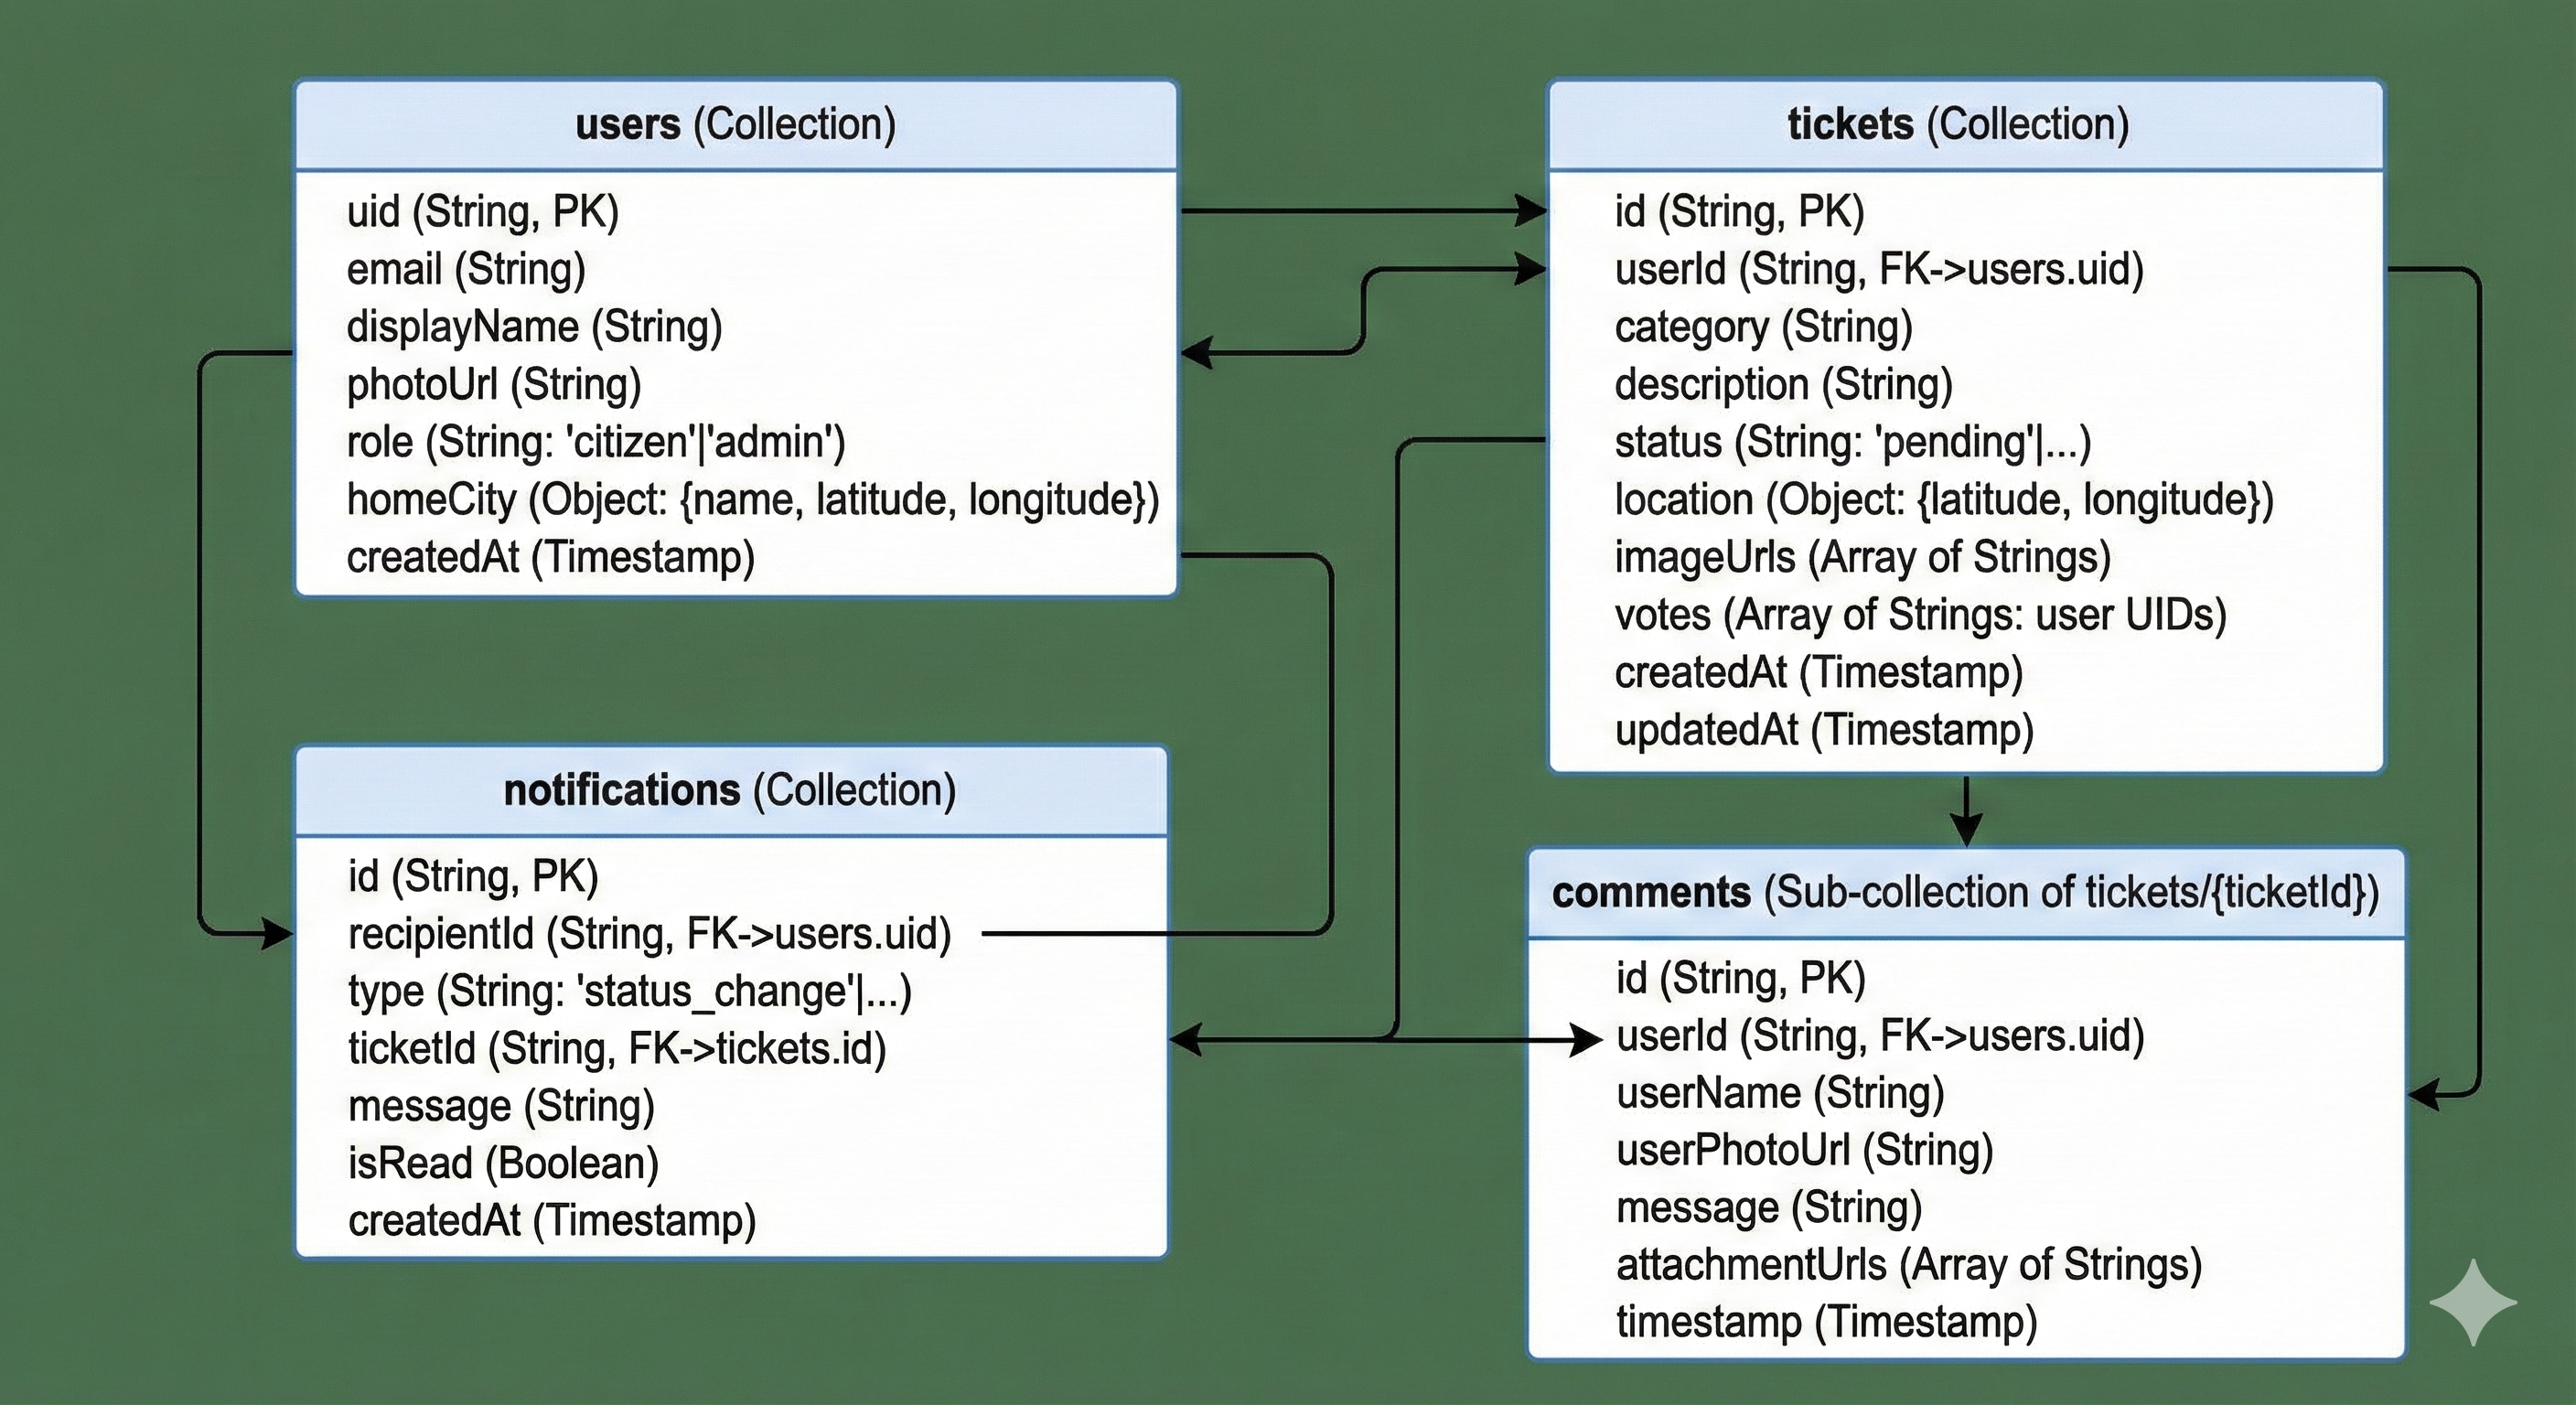
\includegraphics[width=0.8\textwidth]{images/database.png}
    \caption{Schema bazei de date Firestore}
\end{figure}

\subsubsection{1. Colectia: \texttt{users}}
Contine setarile de profil si preferintele de navigare.
\begin{itemize}
    \item \texttt{uid} (String): ID unic.
    \item \texttt{email} (String).
    \item \texttt{displayName} (String).
    \item \texttt{photoUrl} (String): URL catre avatarul stocat in Firebase Storage.
    \item \texttt{role} (String): \textit{'citizen'} sau \textit{'admin'}.
    \item \texttt{homeCity} (Object): Preferinta de localizare (evita geolocatia repetitiva).
        \begin{itemize}
            \item \texttt{name} (String): Ex: "Craiova".
            \item \texttt{latitude} (Number): Coordonata centrala a orasului.
            \item \texttt{longitude} (Number).
        \end{itemize}
    \item \texttt{createdAt} (Timestamp).
\end{itemize}

\subsubsection{2. Colectia: \texttt{tickets}}
Include logica de votare si galerie foto.
\begin{itemize}
    \item \texttt{id} (String): ID unic.
    \item \texttt{userId} (String): Referinta user.
    \item \texttt{category} (String): Ex: 'Gropi', 'Iluminat'.
    \item \texttt{description} (String).
    \item \texttt{status} (String): \textit{'pending', 'approved', 'rejected', 'resolved'}.
    \item \texttt{location} (Object): lat/long.
    \item \texttt{imageUrls} (Array of Strings): Galerie foto (initiala).
    \item \texttt{votes} (Array of Strings): Lista UID-urilor utilizatorilor care au dat "Upvote".
        \begin{itemize}
            \item \textit{Nota:} Numarul de voturi se calculeaza ca \texttt{votes.length}.
        \end{itemize}
    \item \texttt{createdAt}, \texttt{updatedAt} (Timestamp).
\end{itemize}

\subsubsection{3. Sub-colectia: \texttt{tickets/\{ticketId\}/comments}}
\begin{itemize}
    \item \texttt{id}, \texttt{userId}, \texttt{userName} (String).
    \item \texttt{userPhotoUrl} (String): Avatarul autorului (pentru afisare rapida in lista de discutii).
    \item \texttt{message} (String).
    \item \texttt{attachmentUrls} (Array of Strings): Galerie foto (comentarii).
    \item \texttt{timestamp} (Timestamp).
\end{itemize}

\subsubsection{4. Colectia: \texttt{notifications}}
Stocheaza alertele pentru utilizatori.
\begin{itemize}
    \item \texttt{id} (String): ID unic.
    \item \texttt{recipientId} (String): Destinatarul notificarii.
    \item \texttt{type} (String): \textit{'status\_change', 'new\_comment', 'vote\_milestone'}.
    \item \texttt{ticketId} (String): Referinta catre tichet.
    \item \texttt{message} (String): Textul afisat (ex: "Sesizarea ta a fost rezolvata!").
    \item \texttt{isRead} (Boolean): Indicator citit/necitit.
    \item \texttt{createdAt} (Timestamp).
\end{itemize}

\section{Arhitectura Generala a Aplicatiei}

\subsection{Schema Bloc}
\begin{center}
    \fbox{\parbox{0.9\textwidth}{
        \centering
        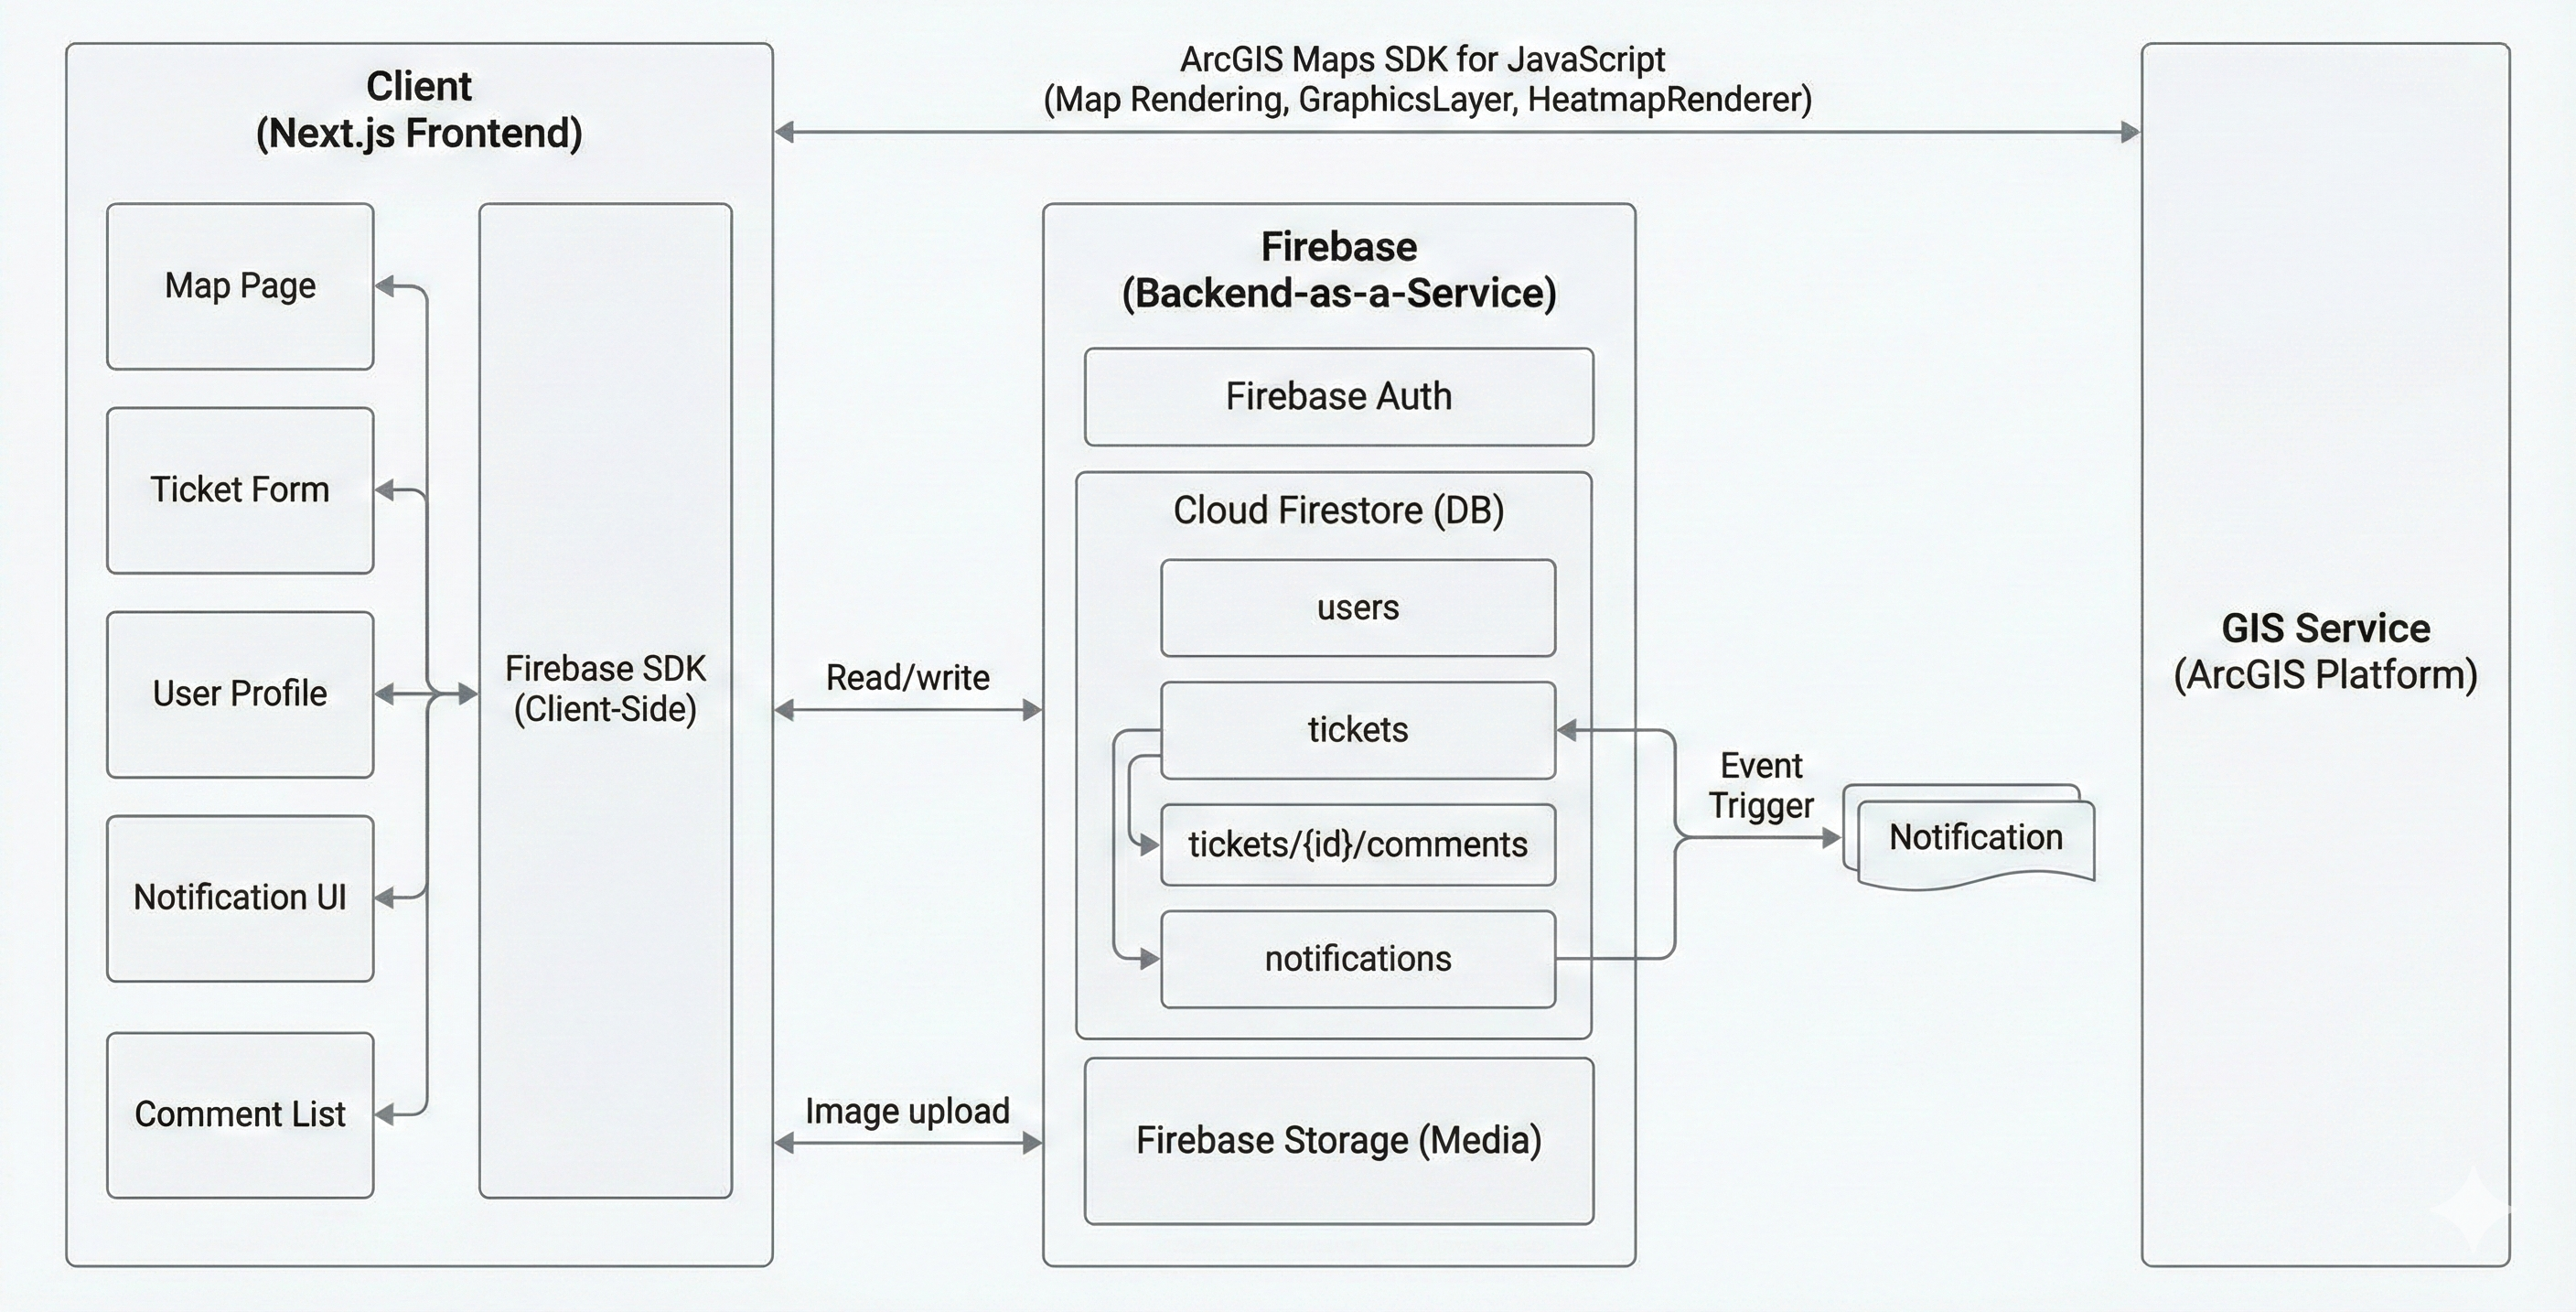
\includegraphics[width=0.9\textwidth]{images/architecture.png}
    }}
\end{center}

\section{Diagrama Cazurilor de Utilizare}

\begin{center}
    \fbox{\parbox{0.9\textwidth}{
        \centering
        \vspace{1cm}
        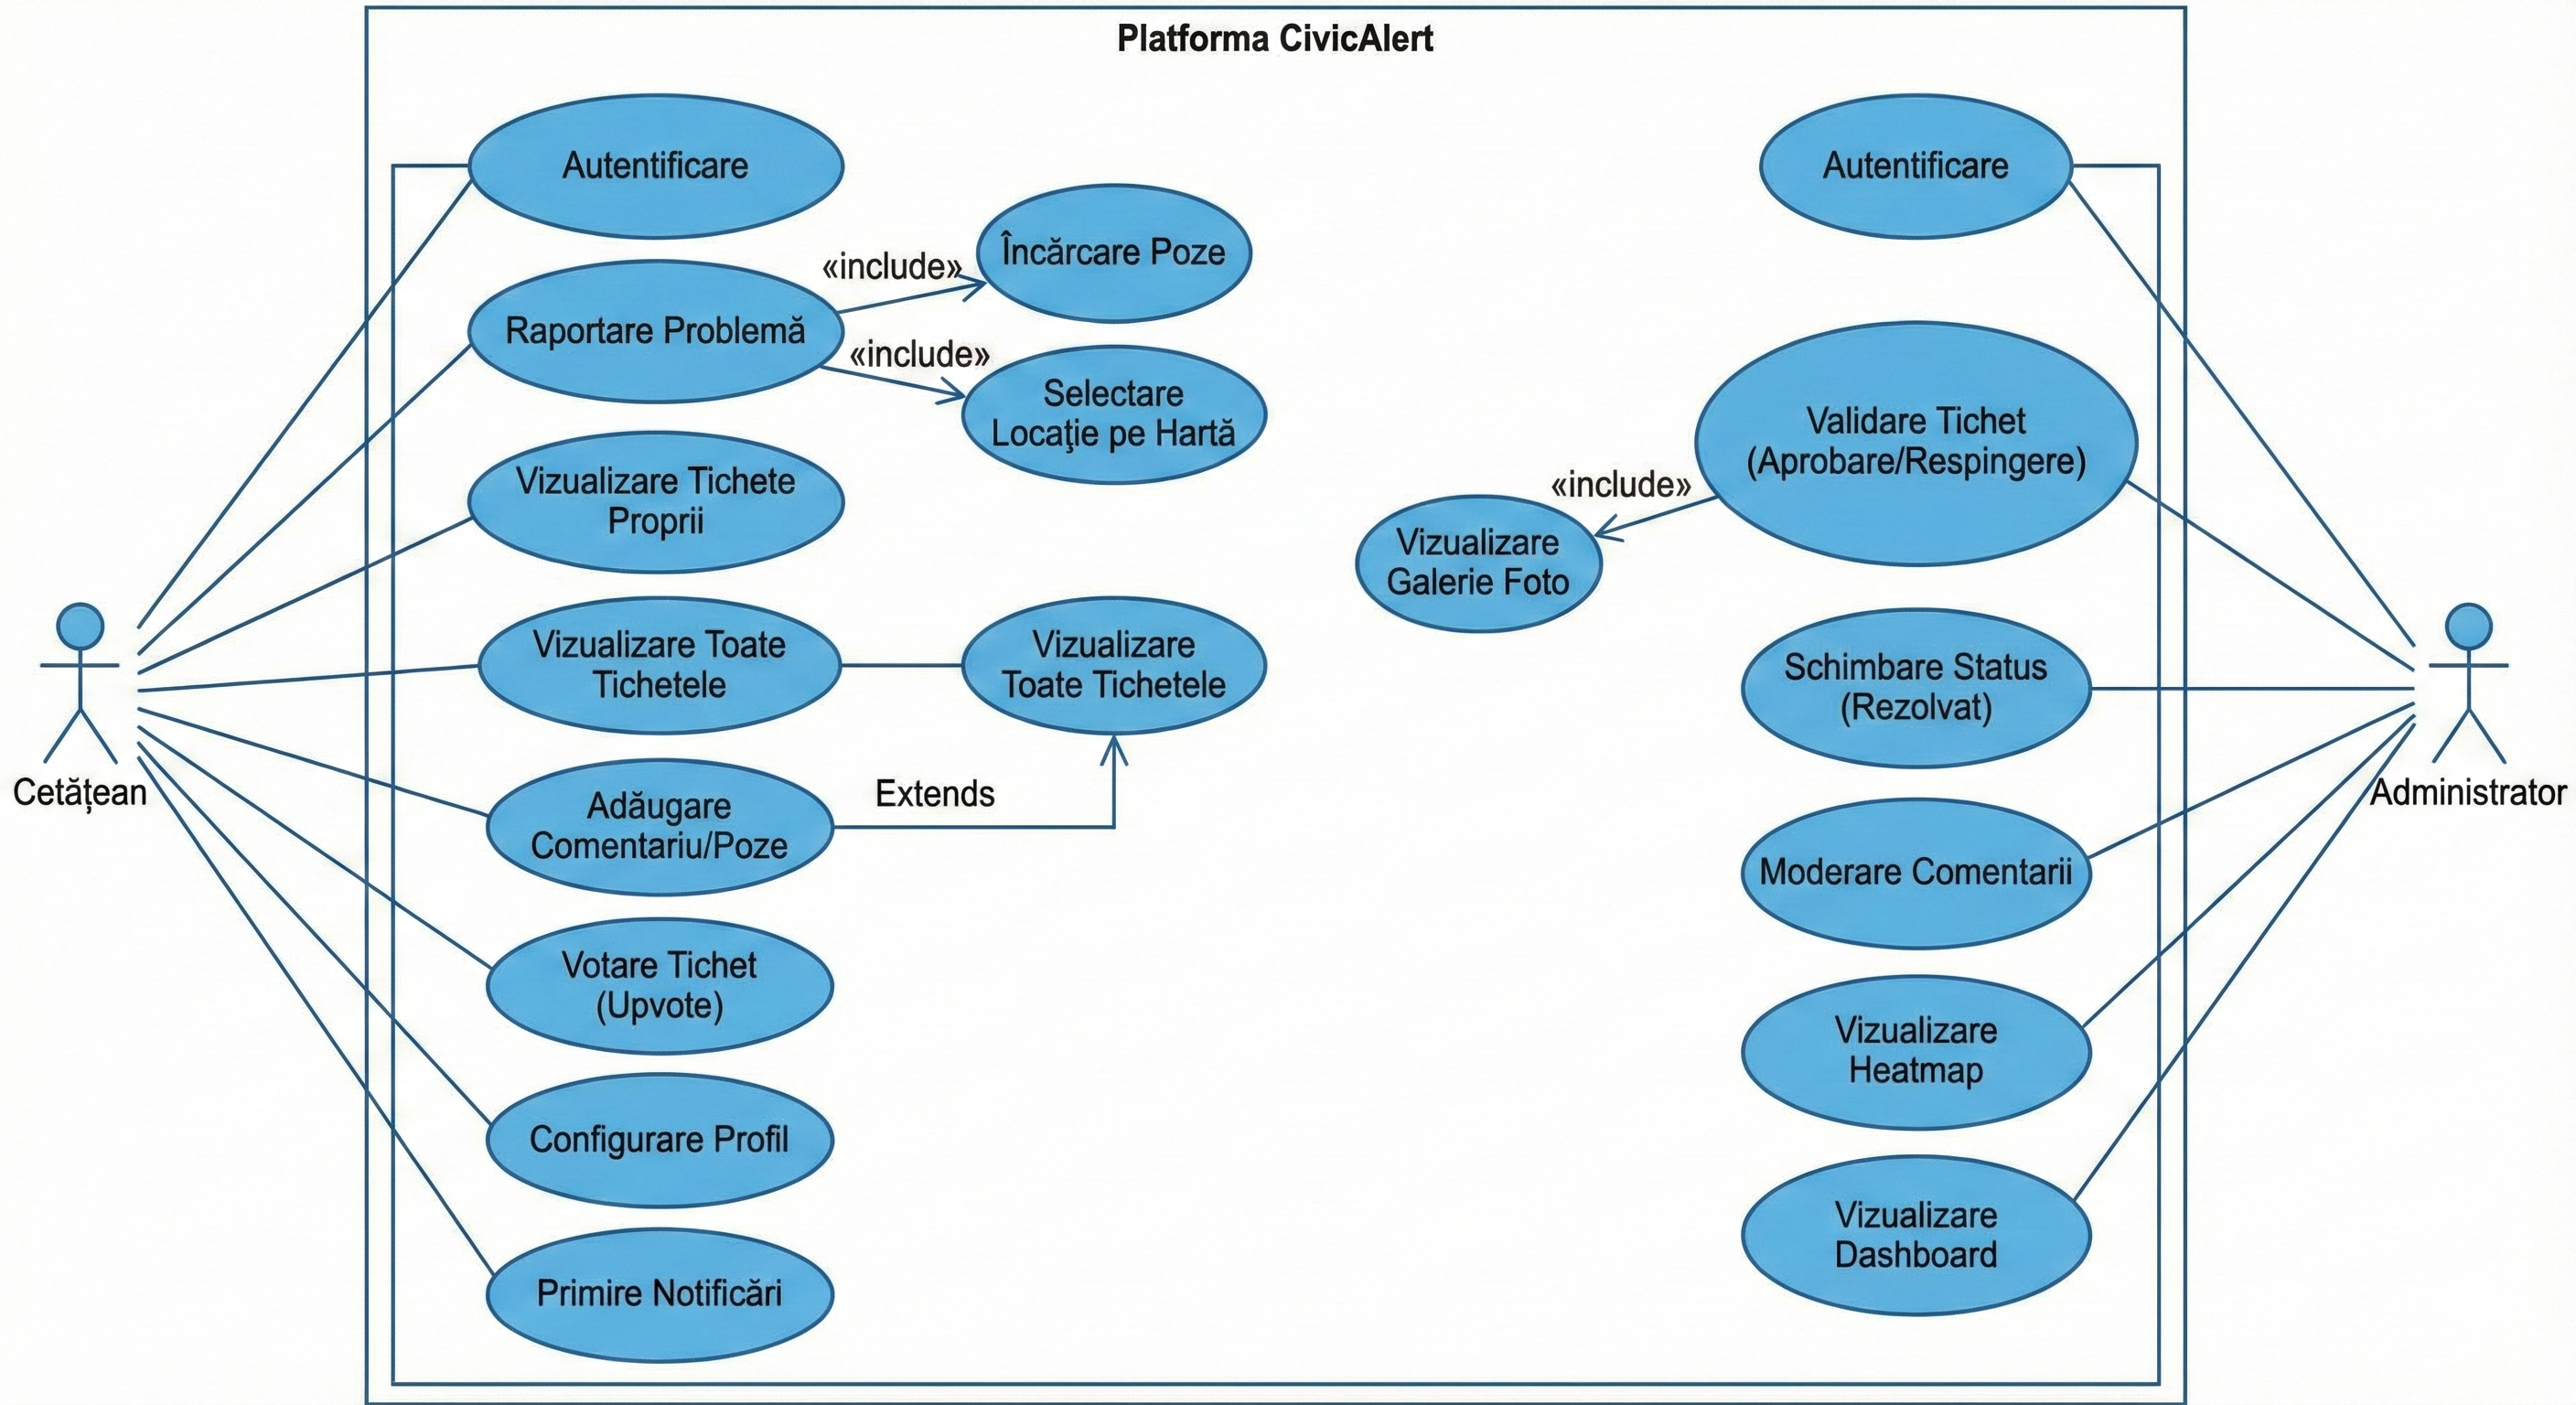
\includegraphics[width=0.9\textwidth]{images/use_cases.png}
        \vspace{1cm}
    }}
\end{center}

\section{Tehnologii}

Aceasta sectiune detaliaza stiva tehnologica aleasa pentru implementarea platformei CivicAlert, justificand alegerile facute in functie de cerintele de performanta, scalabilitate si functionalitatile geospatiale necesare.

\subsection{Generale}
Arhitectura aplicatiei este de tip \textit{Serverless} si \textit{Single Page Application (SPA)} (cu elemente de Server-Side Rendering pentru performanta initiala), bazata pe ecosistemul JavaScript/TypeScript.

\textbf{Tehnologii si Framework-uri Principale:}
\begin{itemize}
    \item \textbf{Frontend Framework: Next.js (React)}
        \begin{itemize}
            \item Folosit pentru construirea interfetei utilizator, gestionarea rutarii si optimizarea performantei prin incarcarea hibrida a paginilor.
            \item Limbajul de programare utilizat este \textbf{TypeScript}, pentru a asigura robustetea codului prin tipizare statica.
        \end{itemize}
    \item \textbf{Backend-as-a-Service (BaaS): Google Firebase}
        \begin{itemize}
            \item Inlocuieste necesitatea unui server backend traditional.
            \item \textbf{Cloud Firestore:} Baza de date NoSQL, orientata pe documente, folosita pentru stocarea tuturor datelor structurate (utilizatori, tichete, comentarii, notificari, voturi).
            \item \textbf{Firebase Authentication:} Gestioneaza intregul flux de autentificare si securitatea conturilor.
            \item \textbf{Firebase Storage:} Stocare de obiecte (bucket) pentru fisierele media (imagini incarcate de utilizatori).
        \end{itemize}
    \item \textbf{Platforma GIS: ArcGIS}
        \begin{itemize}
            \item \textbf{ArcGIS Maps SDK for JavaScript:} Biblioteca principala utilizata pentru toate functionalitatile geospatiale: randarea hartii interactive, afisarea incidentelor si analiza spatiala (heatmap).
            \item \textbf{ArcGIS Online basemaps:} Hartile de fundal (ex: strazile, imaginile satelitare) sunt consumate ca servicii de la Esri.
        \end{itemize}
\end{itemize}

\textbf{Unelte de Dezvoltare si UI:}
\begin{itemize}
    \item \textbf{Tailwind CSS:} Framework CSS \textit{utility-first} pentru stilizarea rapida si responsive a componentelor UI.
    \item \textbf{Node.js \& npm:} Mediul de executie si gestionarul de pachete pentru dependentele proiectului.
    \item \textbf{Git \& GitHub:} Pentru controlul versiunilor si colaborarea in echipa.
\end{itemize}

\section{Organizare Activitati}

\begin{figure}[h!]
    \centering
    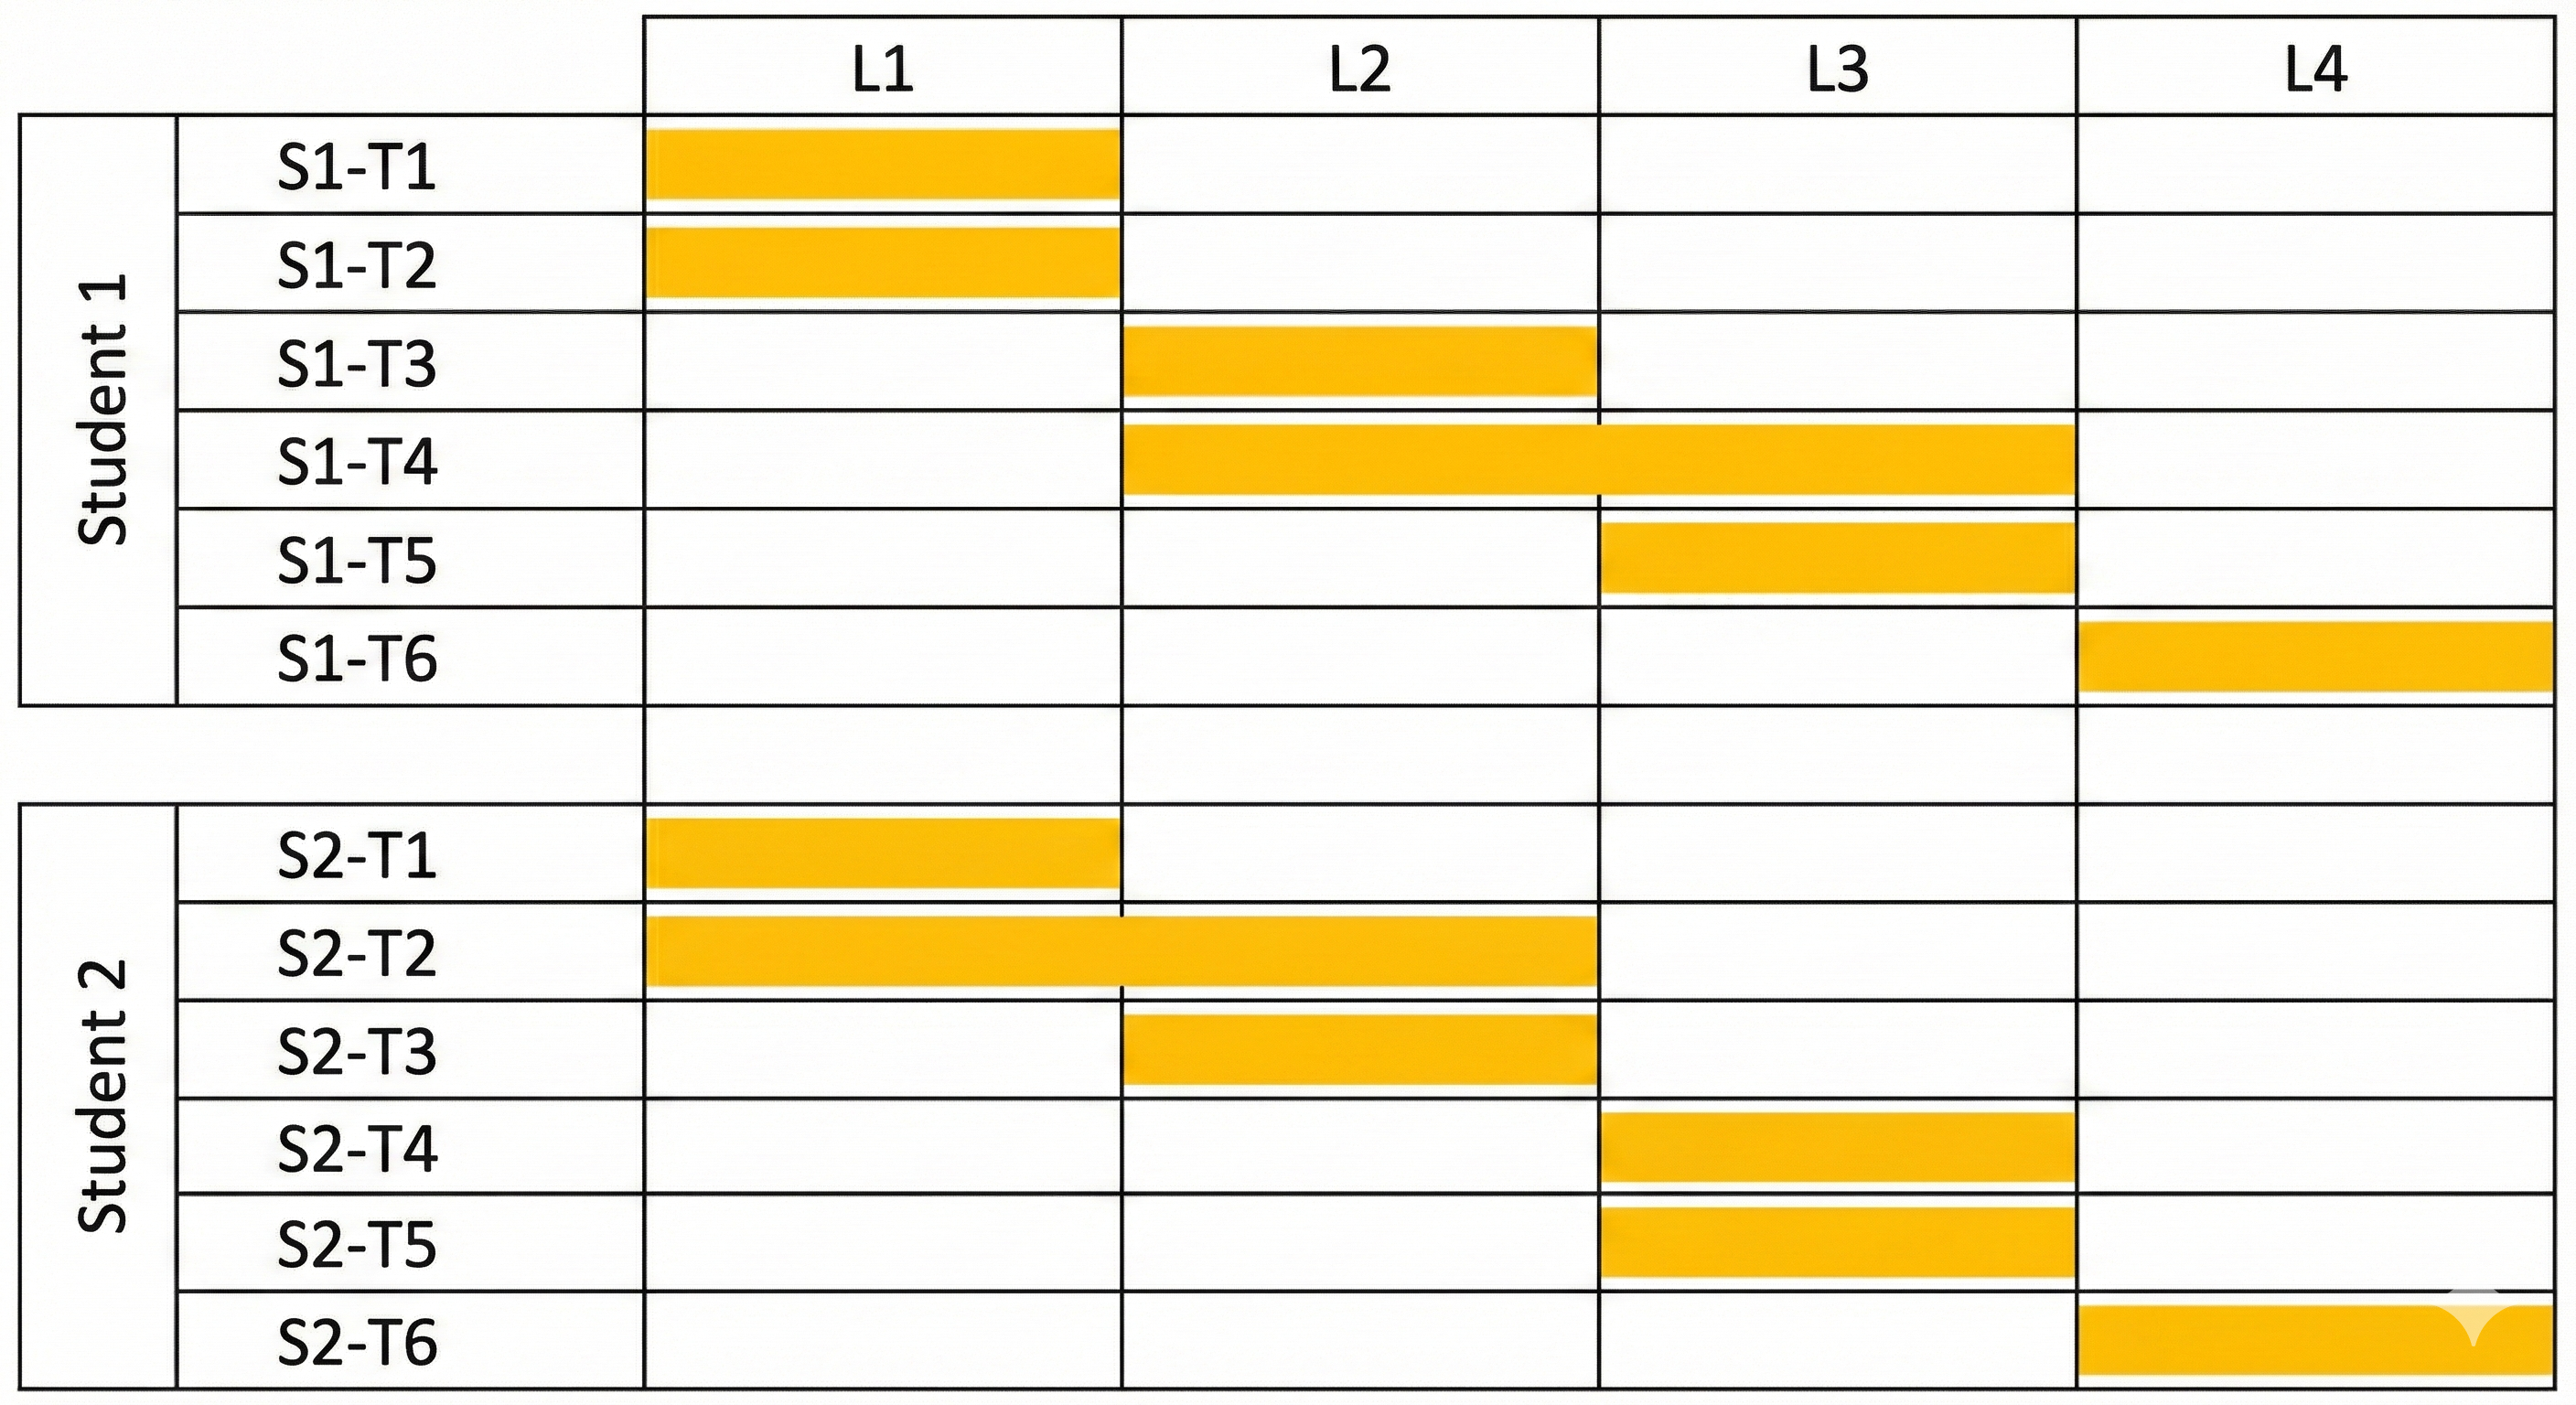
\includegraphics[width=0.9\textwidth]{images/tasks.png} % Asigura-te ca fisierul imagine este in acelasi folder
    \caption{Planificarea task-urilor pe laboratoare}
\end{figure}

\subsubsection*{Legenda Task-uri}

\textbf{Student 1:}
\begin{description}[labelwidth=2cm]
    \item[S1-T1] Configurare Mediu + Autentificare (Login/Register)
    \item[S1-T2] Creare Structura Baza de Date + Pagina Profil
    \item[S1-T3] Integrare Harta Base View (ArcGIS)
    \item[S1-T4] Formular Tichet + Upload Multiplu Poze
    \item[S1-T5] Implementare Centrare Harta pe Orasul Userului
    \item[S1-T6] Creare Componenta Sidebar Listare Tichete
\end{description}

\textbf{Student 2:}
\begin{description}[labelwidth=2cm]
    \item[S2-T1] Conversie Date Firestore in ArcGIS Graphics
    \item[S2-T2] Implementare si Configurare Pop-ups (cu Galerie Foto)
    \item[S2-T3] Creare Dashboard Administrator
    \item[S2-T4] Implementare Heatmap Renderer
    \item[S2-T5] Implementare Sistem de Votare (Upvote)
    \item[S2-T6] Dezvoltare Modul Comentarii si Notificari
\end{description}

\section{Identificarea Riscurilor}

Analiza riscurilor a fost efectuata pe baza unei matrici de tip \textit{Probabilitate vs. Impact}, pentru a prioritiza masurile de preventie.

\begin{figure}[h!]
    \centering
    % Asigura-te ca imaginea 3x3 este salvata cu acest nume
    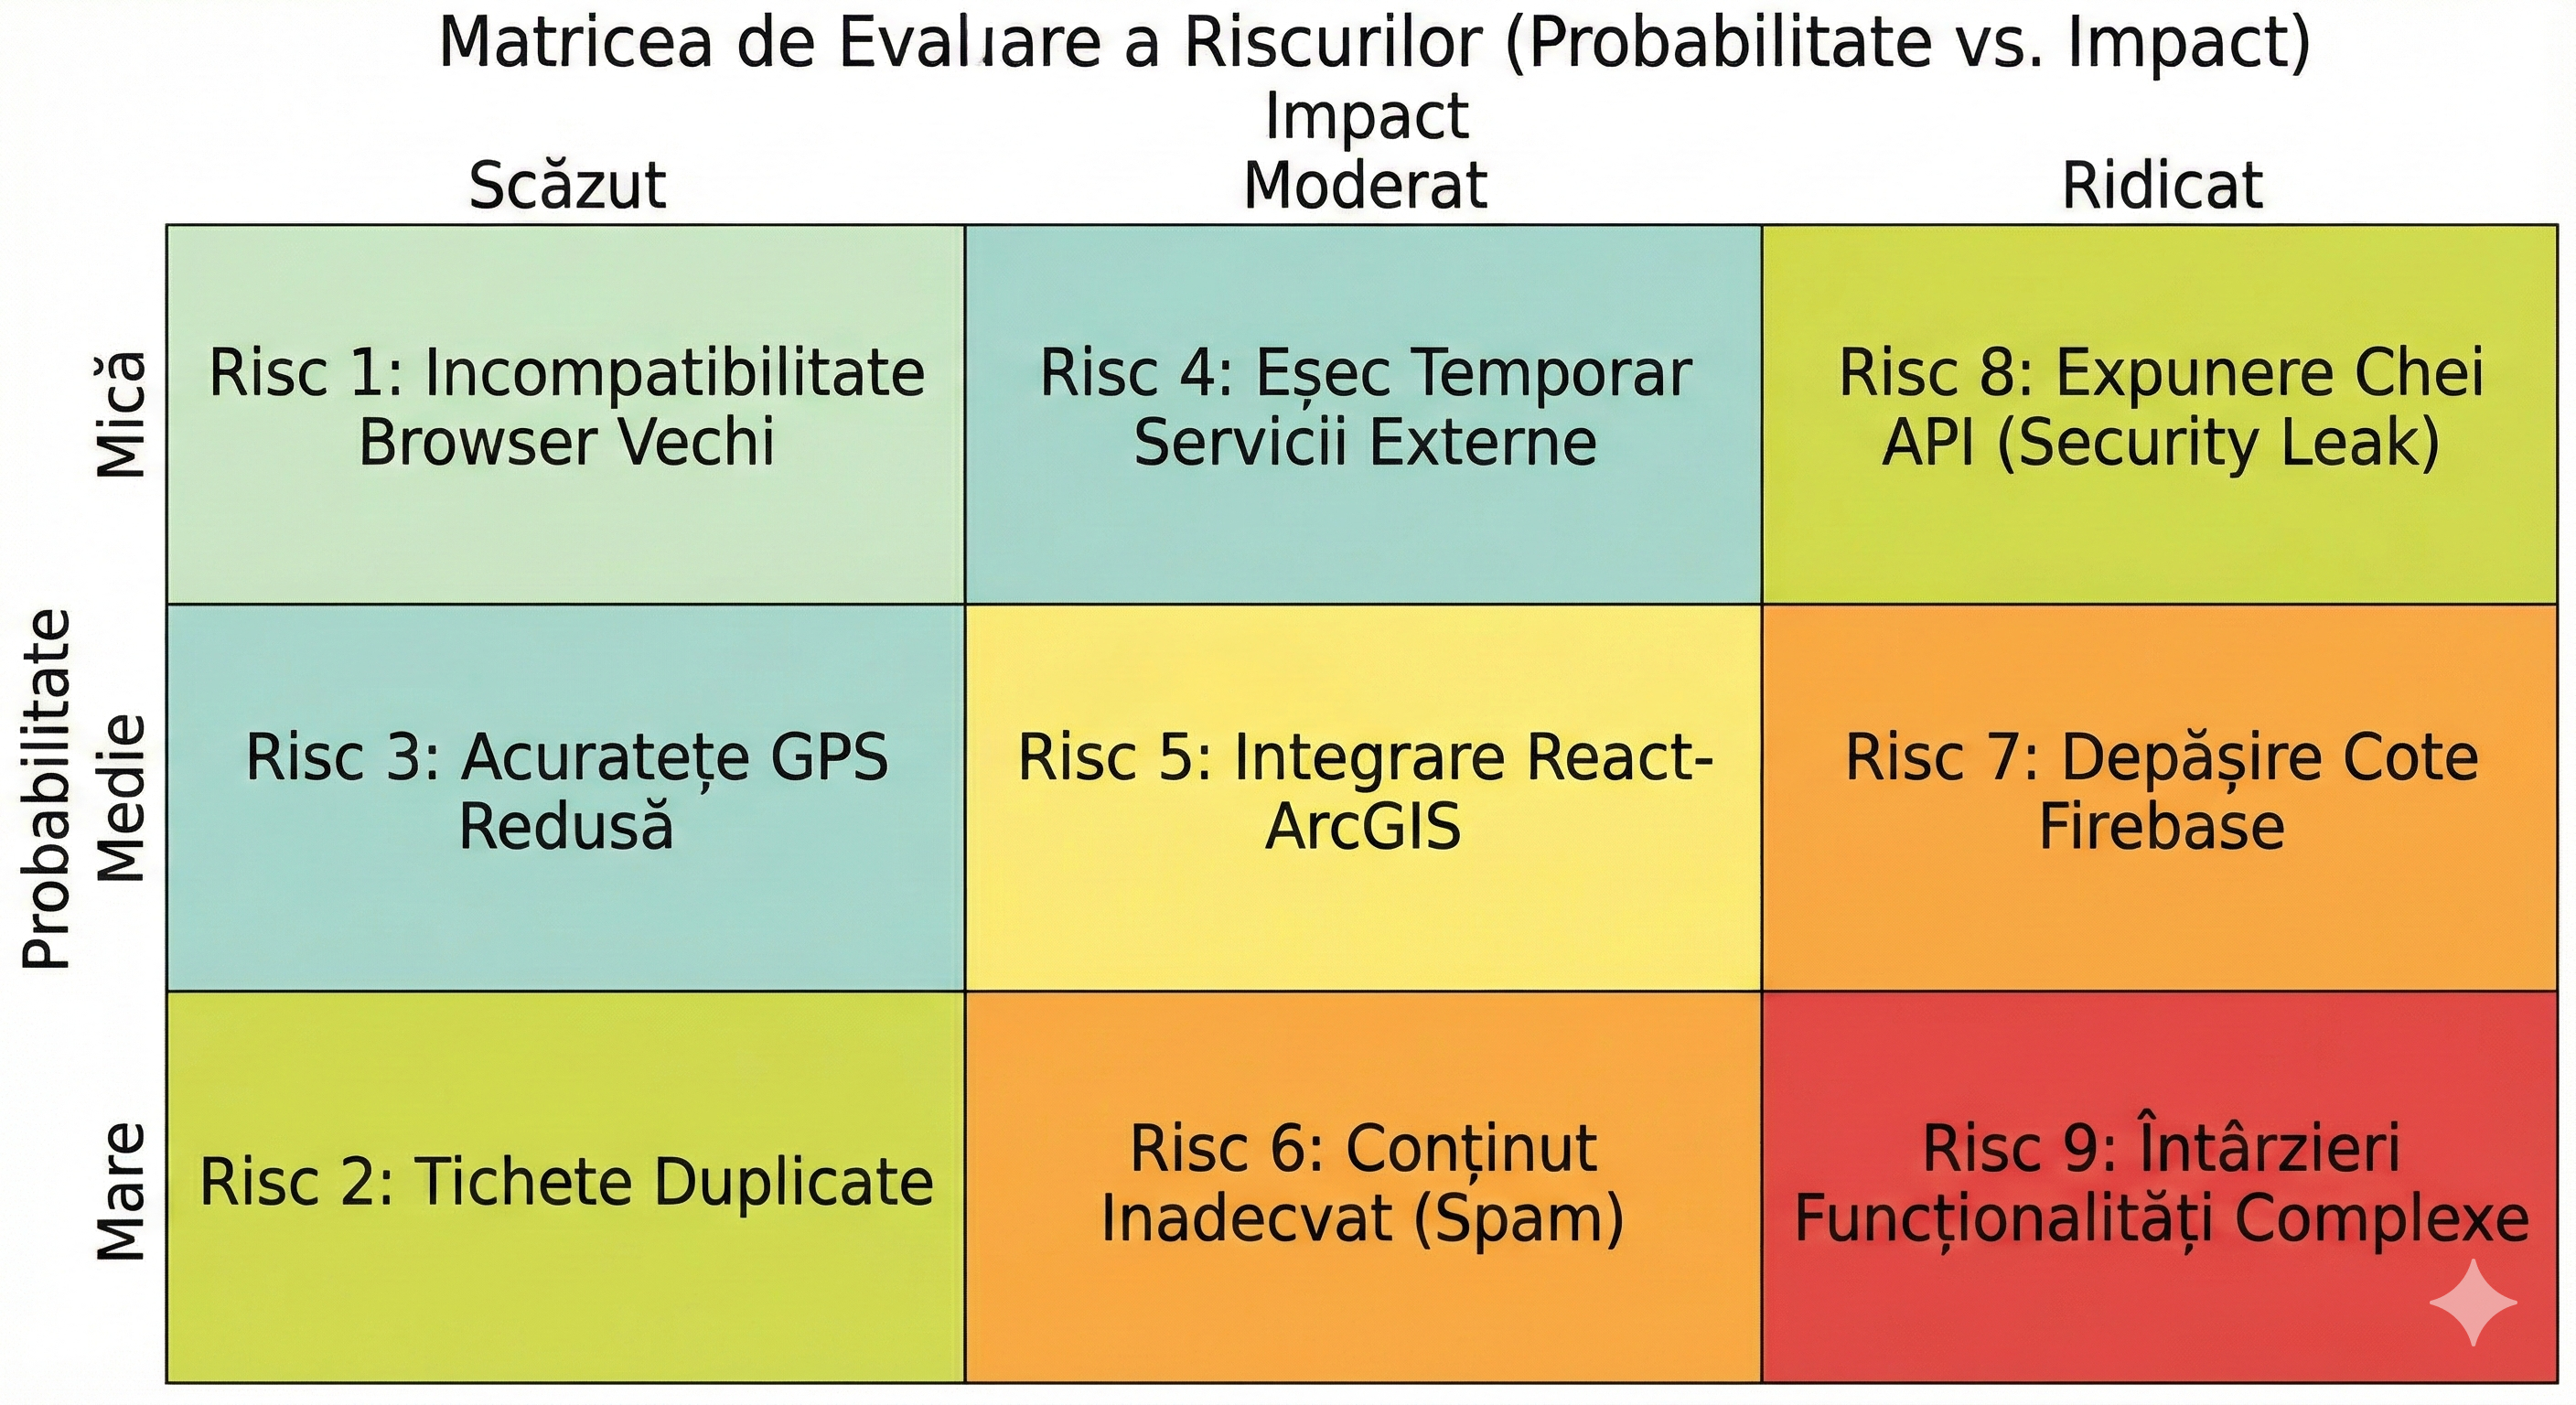
\includegraphics[width=0.75\textwidth]{images/risks.png} 
    \caption{Matricea de evaluare a riscurilor (Probabilitate vs. Impact)}
\end{figure}

\subsection*{Catalogul Riscurilor si Planul de Mitigare}

Tabelul urmator detaliaza cele 9 riscuri identificate in matricea de mai sus si solutiile tehnice propuse pentru fiecare.

\vspace{0.5cm}

% Setari pentru spatierea in tabel
\renewcommand{\arraystretch}{1.4} 

% Inceputul mediului longtable
\begin{longtable}{|p{1.8cm}|p{6.6cm}|p{6.6cm}|}
\hline
\textbf{Cod Matrice} & \textbf{Descriere Risc} & \textbf{Masuri de Contracarare} \\ \hline
\endfirsthead % Antetul pentru prima pagina a tabelului

% Antetul care se repeta daca tabelul trece pe pagina urmatoare
\multicolumn{3}{c}%
{{\bfseries \tablename\ \thetable{} -- continuare din pagina anterioara}} \\
\hline
\textbf{Cod Matrice} & \textbf{Descriere Risc} & \textbf{Masuri de Contracarare} \\ \hline
\endhead

% Subsolul paginii (daca tabelul continua)
\hline \multicolumn{3}{|r|}{{Continua pe pagina urmatoare...}} \\ \hline
\endfoot

% Subsolul ultimei pagini a tabelului
\hline
\endlastfoot

% --- CONTINUTUL TABELULUI ---
\textbf{Risc 1} & \textbf{Incompatibilitate Browser Vechi} \newline (Probabilitate Mica / Impact Scazut) \newline Un numar mic de utilizatori ar putea accesa platforma de pe browsere care nu suporta WebGL (necesar ArcGIS) sau ES6+. & Afisarea unui mesaj proactiv ("Banner") pentru utilizatorii detectati cu browsere incompatibile, recomandand actualizarea la una moderna (Chrome, Firefox, Edge). \\ \hline

\textbf{Risc 2} & \textbf{Tichete Duplicate} \newline (Probabilitate Mare / Impact Scazut) \newline Probabilitate mare ca vecinii sa raporteze independent aceeasi problema (ex: o groapa). & Implementarea functiei de \textbf{"Upvote"} (Sustinere). Utilizatorul vede pin-ul existent si apasa "Sustin" in loc sa creeze un tichet nou. \\ \hline

\textbf{Risc 3} & \textbf{Acuratete GPS Redusa} \newline (Probabilitate Medie / Impact Scazut) \newline Semnalul GPS al telefonului/browserului poate avea abateri de 10-50m. & Posibilitatea de ajustare manuala a pozitiei marker-ului pe harta (\textit{Drag \& Drop}) inainte de trimiterea formularului. \\ \hline

\textbf{Risc 4} & \textbf{Esec Temporar Servicii Externe} \newline (Probabilitate Mica / Impact Moderat) \newline Intreruperi rare ale API-urilor Esri (ArcGIS Online) sau Google Firebase. & Implementarea unei tratari elegante a erorilor (Graceful Degradation) in UI (ex: afisarea unui mesaj "Harta este momentan indisponibila" in loc de blocarea aplicatiei). \\ \hline

\textbf{Risc 5} & \textbf{Integrare React-ArcGIS} \newline (Probabilitate Medie / Impact Moderat) \newline Dificultati in sincronizarea starii React cu DOM-ul hartii ArcGIS (risc de memory leaks). & Utilizarea \textit{React Hooks} (`useEffect`, `useRef`) pentru a gestiona strict ciclul de viata al hartii si distrugerea instantei la unmount. \\ \hline

\textbf{Risc 6} & \textbf{Continut Inadecvat (Spam)} \newline (Probabilitate Mare / Impact Moderat) \newline Incarcarea de imagini irelevante sau limbaj ofensator in comentarii. & Implementarea unui buton de "Raporteaza" si a unui panou de moderare pentru Admin (stergere continut). \\ \hline

\textbf{Risc 7} & \textbf{Depasire Cote Firebase} \newline (Probabilitate Medie / Impact Ridicat) \newline Atingerea limitelor planului gratuit (Spark) din cauza numarului mare de citiri. & Optimizarea interogarilor (paginare, limitare rezultate) si stocarea datelor statice (ex: lista orase) in cache local. \\ \hline

\textbf{Risc 8} & \textbf{Expunere Chei API (Security Leak)} \newline (Probabilitate Mica / Impact Ridicat) \newline Includerea accidentala a cheilor private (ex: Firebase Service Account) in codul client-side. & Utilizarea stricta a variabilelor de mediu (`.env.local`) si asigurarea ca cheile sensibile sunt accesate doar din API Routes (server-side), nu din browser. \\ \hline

\pagebreak % Optional: Fortam trecerea ultimului risc pe pagina noua daca e cazul

\textbf{Risc 9} & \textbf{Intarzieri Functionalitati Complexe} \newline (Probabilitate Mare / Impact Ridicat) \newline Riscul de a nu finaliza Heatmap-ul sau Votarea la timp. & Prioritizarea modulelor critice (MVP) si simplificarea cerintelor (ex: Heatmap static in loc de dinamic) daca este necesar. \\
\end{longtable}

\end{document}